% CONTAINDER --- Elsevier IJCIP submission build (elsarticle, single column).
% The IEEEtran build (main.tex) is retained unchanged; this file targets IJCIP.
% 'review' option gives the double-spaced, line-numbered format Elsevier expects.
\documentclass[review]{elsarticle}

\usepackage{amsmath,amssymb}
\usepackage{booktabs}
\usepackage{graphicx}
\usepackage{url}

% Custom macros for the four radii (single source of notation truth).
\newcommand{\BRreach}{\mathrm{BR}_{\mathrm{reach}}}
\newcommand{\BRflex}{\mathrm{BR}_{\mathrm{flex}}}
\newcommand{\BRauth}{\mathrm{BR}_{\mathrm{auth}}}
\newcommand{\BRexp}{\mathrm{BR}_{\mathrm{exp}}}
\newcommand{\BRphys}{\mathrm{BR}_{\mathrm{phys}}}
\newcommand{\Reach}{\mathrm{ReachSet}}

\journal{International Journal of Critical Infrastructure Protection}

\begin{document}

\begin{frontmatter}

\title{CONTAINDER: Bounding Credential-Compromise Impact in
IEEE~2030.5 DER Systems}

\author{Huan Bui\corref{cor1}}
\ead{hbui11@charlotte.edu}
\cortext[cor1]{Corresponding author.}
\affiliation{organization={University of North Carolina at Charlotte},
             city={Charlotte}, state={NC}, country={USA}}

\begin{abstract}
The IEEE~2030.5 standard governs communication with distributed energy resources (DERs), but its
trust model binds a device's long-lived bootstrap identity to its operational authorization and
forbids online certificate revocation, so a stolen credential retains control authority for a
lifetime the standard permits to be indefinite. We argue that the harm of such a compromise is
not captured by static reachability, and introduce a four-dimension model separating cyber reach,
state-dependent commandable flexibility, retained authority, and feeder consequence; a worked
counterexample gives two compromises with identical reach yet different flexibility, persistence,
and feeder outcome. Guided by the model, CONTAINDER replaces the conflated device credential with
attested, short-lived, scope-bound operational credentials, using non-renewal rather than
revocation for containment, with incremental deployment through native and gateway-proxy tiers. We
build a working credential service with real X.509 and mutual TLS and a real feeder power-flow
pipeline, and report a preliminary evaluation on the IEEE~8500-node feeder: ten security invariants
hold, per-command enforcement bounds authority at credential expiry, attested issuance costs about
$0.2$\,ms, and narrowing authorization keeps a compromise's induced overvoltage within limits where
a legacy credential drives it far outside. These reduced-scale results precede the full
pre-registered evaluation.
\end{abstract}

\begin{keyword}
Critical infrastructure protection \sep distributed energy resources \sep IEEE~2030.5 \sep
remote attestation \sep authorization \sep cyber-physical security
\end{keyword}

\end{frontmatter}

\section{Introduction}

% provenance: dec_01KXT240A70R8N104BPN5G07CJ (RQ1) motivates the reach/scope question.
Distributed energy resources now participate in grid operations at a scale that makes their
control interface a systemic concern. IEEE~2030.5 (Smart Energy Profile~2.0), profiled for
distribution use by the Common Smart Inverter Profile (CSIP), is the application protocol through
which utilities and aggregators dispatch inverter-based resources. An adversary who obtains a
credentialed identity in this ecosystem does not merely read data; it commands real and reactive
power on physical hardware connected to the grid.

% provenance: jrn_01KXT3JPAZ8RSGZK99X4G3HWPE (SAND2019-1490 4.1) supports the two facts here.
Two properties of the trust model make this harder than a conventional credential-theft problem.
The device's bootstrap identity and its operational authorization are the same certificate, so
there is no separate short-lived credential to lose. And that certificate does not expire and
cannot be revoked: the analysis of record for these standards states that the PKI is distinguished
by ``the use of non-expiring certificates and the explicit prohibition of CRL and OCSP'', and that
``if the device's private key is compromised, the device certificate cannot be
revoked''~\cite{obert2019recommendations}. What the standard offers instead is a local allow or
deny list.

The obvious objection is that a denylist is enough --- the operator refuses the compromised
identity and the incident is over. \textbf{We measure that assumption and it does not hold.}
Denying the identity of an adversary who is already connected reduces integrated feeder harm by
\emph{exactly zero} on both feeders we evaluate. It refuses new sessions, which is all it claims
to do; the adversary's established session continues to issue commands, and the scheduled control
it has already installed continues to act on the inverter. Containment fails not because authority
cannot be withdrawn but because withdrawing it at one layer leaves two others running.

That observation organises the paper. Bounding a DER compromise requires controlling two
independent quantities: the \emph{set of physical actions} an authorization admits, and the
\emph{duration} for which authority remains effective at every layer that can carry it --- the
credential, the open session, and the issued command.

CONTAINDER separates bootstrap identity from short-lived, attested, scope-bound operational
authority, and enforces expiry at all three layers. Because grid actuation persists in a way
computation does not, expiry that stops at the credential is not containment: we show that a
credential lifetime with neither session nor command enforcement removes no harm at all, and that
command cleanup without session enforcement removes none either, because the adversary re-issues
over the session that is still open.

\subsection*{Contributions}
\begin{itemize}
\item \emph{A DER credential and enforcement architecture} that separates bootstrap identity,
operational credential and value-constrained authorization, and enforces expiry at the credential,
session and command-effect layers, deployable through a gateway proxy that leaves downstream
IEEE~2030.5 endpoints unmodified.

\item \emph{A measurement of what each containment layer is worth.} Identity denial alone removes
$0\%$ of integrated harm; adding session termination removes $48.8$--$54.4\%$; adding command
cancellation removes $70.6$--$76.3\%$. The two enforcement mechanisms fail alone for different
reasons and are separately necessary --- a claim an earlier version of this work asserted from a
harness that could not identify it, and which is here earned from a lifecycle model that
distinguishes the three layers.

\item \emph{An authorization-shape result, with the condition under which it matters.} At
identical width, a reactive bound that admits zero absorption fails to contain where an absorption
floor contains, at negligible cost to volt-var service. The magnitude of that effect scales with
the reactive absorption the feeder is actually drawing rather than with PV penetration; it
survives at an operating point where legitimate operation is compliant, but is an order of
magnitude smaller there than at an overstressed one.

\item \emph{A corrected, released evaluation harness} on two public feeders, with a
pre-registration committed to version control before any treatment arm ran, every departure from
it disclosed, and two defects in the predecessor harness identified and repaired.
\end{itemize}

We claim no novelty for short-lived certificates or for expiry-based containment. The Web PKI
ratified that trade in 2023~\cite{cabf-sc063v4}, and the Sandia analysis of these very standards
recommends limited-life certificates and records that manufacturers are ``not required to limit
the life of a device certificate''~\cite{obert2019recommendations} --- which makes a short-lived
operational credential permitted rather than new. What is new here is the mapping onto DER
authorization: which layers expiry must reach before it contains anything, which control point an
authorization must withhold, and the operating condition that decides whether either matters.

\section{Background and Threat Model}\label{sec:threat}

\subsection{Authorization in IEEE~2030.5 / CSIP}
% provenance: jrn_01KXT490ZD4444AWMRG5296GJA (threat model + CSIP function sets); lit passos2025tutorial.
IEEE~2030.5 uses mutual TLS with X.509 device certificates. A device's identity is the
certificate-derived LFDI/SFDI, and its authorization is scoped by a
\texttt{FunctionSetAssignments} resource binding it to one or more \texttt{DERProgram}s.
Physical control authority is carried by the \texttt{DERControlBase} modes: active-power capping
(\texttt{opModMaxLimW}), signed fixed active power (\texttt{opModFixedW}), reactive power
(\texttt{opModFixedVar}, \texttt{opModVoltVar}), volt-watt and frequency-watt curves, and the hard
connect and energize controls~\cite{passos2025tutorial}. The standard specifies certificate-based
authentication and function-set scoping; it does not mandate a single canonical access-control
object, and no accessible source establishes that it can bound the \emph{value} a control may
take. That distinction is where our design sits, and Section~\ref{sec:design} states it plainly
rather than implying native expressiveness.

\subsection{Six ways authority can be withdrawn, and what each reaches}
The literature tends to treat ``revocation'' as one thing. It is six, and they terminate different
layers, which is the whole reason a compromise can outlive the response to it:

\begin{enumerate}\itemsep2pt
\item \emph{PKI revocation} --- a CRL or OCSP status marks the certificate invalid.
\item \emph{Local identity denial} --- the server refuses the certificate-derived identity.
\item \emph{Authorization removal} --- \texttt{FunctionSetAssignments} or \texttt{DERProgram}
      membership changes.
\item \emph{Session termination} --- an established authenticated channel is closed or forced to
      revalidate.
\item \emph{Command cancellation} --- a scheduled or latched \texttt{DERControl} is withdrawn,
      superseded, or replaced by a safe default.
\item \emph{Identity replacement} --- the device is re-enrolled or re-keyed.
\end{enumerate}

Only the first is unavailable by construction. The motivating claim of this paper is therefore not
that IEEE~2030.5 offers no way to withdraw authority --- it offers the second, and CSIP builds
enrollment on it --- but that \textbf{the end-to-end time from deciding to contain a compromise to
the cessation of all effective physical authority is not bounded by any of them individually}.
Denying an identity refuses future authorization. On its own it neither closes an open session nor
retracts a control already issued, and Section~\ref{sec:results} measures how much of an attack
survives it.

\subsection{What the accessible standards material establishes}
% provenance: jrn_01KXT3JPAZ8RSGZK99X4G3HWPE (SAND2019-1490 4.1, primary-sourced, full text).
Certificate management differs across editions: IEEE~2030.5-2018~\cite{ieee20305-2018},
IEEE~2030.5-2023~\cite{ieee20305-2023} (which supersedes it, published December 2024), and the
profile in force~\cite{sunspec2018csip}. \textbf{We were unable to obtain IEEE~2030.5-2023.} It is
paywalled at roughly US\$255 and is not in the IEEE GET programme. Every claim below is evidenced
against the 2018 edition and the Sandia analysis of it~\cite{obert2019recommendations}, whose full
text is freely available; Table~\ref{tab:standards} gives each claim its source and its exposure,
and Section~S1 of the supplement reproduces the supporting quotations.

Three points are settled by that material and matter to the design.

\emph{Certificates do not expire, and revocation is prohibited for IEEE~2030.5 certificates.} The
Sandia analysis states that the PKI is distinguished by ``the use of non-expiring certificates and
the explicit prohibition of CRL and OCSP'', that ``once issued, a device certificate has an
indefinite lifetime'', and that ``if the device's private key is compromised, the device
certificate cannot be revoked''~\cite{obert2019recommendations}. The prohibition is specific:
OCSP ``may only be used to verify non-IEEE~2030.5 certificates''. We state the qualification
because an unqualified claim that the protocol forbids OCSP outright is wrong.

\emph{Local allow/deny listing is the sanctioned substitute, and is weaker than revocation.} It is
permitted, not required. The same analysis is explicit about its limits: ``a blacklist is
essentially a local CRL but without the process, rigor and verification behind its issuance'', and
``it is possible for a stolen device certificate that was disallowed in one region to be used in a
different region to gain access because it was only locally blacklisted''.

\emph{A short-lived operational credential is permitted, not prohibited.} Manufacturers following
the guidance ``are not required to limit the life of a device certificate''. Limited-life
certificates are in fact recommended, at a one-year renewal interval. CONTAINDER's contribution is
therefore not the short lifetime, which is neither novel nor disallowed, but the enforcement of
expiry at the session and command-effect layers, on which the accessible material is silent.

\begin{table}[t]
\centering
\caption{Standards claims the argument uses, the free source of record, and residual exposure.
SAND = Sandia SAND2019-1490~\cite{obert2019recommendations}, full text public; CSIP = Common
Smart Inverter Profile v2.1~\cite{sunspec2018csip}. \textbf{No row has been checked against
IEEE~2030.5-2023}, which could not be obtained.}
\label{tab:standards}
\footnotesize
\begin{tabular}{@{}p{0.04\columnwidth}p{0.36\columnwidth}p{0.24\columnwidth}p{0.22\columnwidth}@{}}
\toprule
ID & Claim & Free source & Residual risk \\
\midrule
S1 & Device certificate lifetime indefinite & SAND \S4.1, \S6.4, verbatim & 2023 clause unread \\
S2 & CRL prohibited for 2030.5 certificates & SAND \S4.1, verbatim & 2023 clause unread \\
S3 & OCSP prohibited \emph{for 2030.5 certificates}; permitted for others & SAND \S6.4, verbatim &
2023 clause unread \\
S4 & Local allow/deny listing permitted, not required, and unsynchronised & SAND \S4.1, \S4.1.2 &
low \\
S5 & Short-lived operational credential permitted & SAND \S6.4, verbatim & low \\
S6 & LFDI/SFDI derives from certificate & SAND \S3.1.1; CSIP \S5.2.1.2 & low; two sources \\
S7 & FunctionSetAssignments scopes \emph{functions}; numeric value bounds not established &
CSIP \S5.2.3.1 & \textbf{design depends on it}; see \S\ref{sec:design} \\
S8 & Scheduled DER controls persist & CSIP \S4.4.2, \S6.1.8.2 & \textbf{high}; 2023 drops
mandatory DERControl modes \\
\bottomrule
\end{tabular}
\end{table}

\subsection{Three separated layers}
We separate three layers the baseline conflates. \emph{L1, bootstrap identity}: the
hardware-rooted device certificate. \emph{L2, operational credential}: what authorizes live
sessions to an aggregator or DER management system. \emph{L3, authorization scope}: the
server-side binding from an identity to the function sets and values it may invoke. In baseline
IEEE~2030.5, L1 and L2 are the same indefinitely valid certificate, with no attestation gate. That
conflation, not any cryptographic weakness, is what makes a compromise persist.

\subsection{Compromise classes and what bounds each}
Retained authority differs by compromise class, and reporting one figure for all of them is the
error the pilot made. Table~\ref{tab:classes} gives the classes, the mechanism that bounds each,
and the resulting expectation. The derivations and their Monte-Carlo checks are in
\texttt{pkimodel/retention.py} and \texttt{tests/test\_retention.py}.

Two entries deserve emphasis because an earlier version of this paper got them wrong. For a
\emph{copied operational key} held by an adversary who is not resident on the device, attestation
has nothing to detect: renewal mints a fresh key whether or not anything is found, so retention is
bounded by the remaining epoch at $T/2$ in expectation, \emph{independently of the detection
probability}. For a \emph{persistent} compromise re-checked at each renewal with probability $p$,
the familiar $T/p$ holds only when the compromise arrives immediately after an issuance; under
uniform arrival within the epoch the expectation is $T(1/p - 1/2)$. At $T = 6$\,h and $p = 0.2$,
reporting $T/p$ for a copied key claims $30$\,h of retention where the true expectation is $3$\,h.

\begin{table}[t]
\centering
\caption{Compromise classes, the mechanism that bounds each, and expected retained authority.
$T$ is the credential lifetime and $p$ the per-renewal detection probability. Arrival is uniform
within the epoch unless stated.}
\label{tab:classes}
\footnotesize
\begin{tabular}{@{}p{0.30\columnwidth}p{0.34\columnwidth}p{0.24\columnwidth}@{}}
\toprule
Compromise class & Bounding mechanism & Expected retention \\
\midrule
Copied operational key & fresh key each epoch & $T/2$; \emph{independent of $p$} \\
Persistent, attested & attestation-gated renewal & $T(1/p - 1/2)$ \\
Persistent, unmeasured & none; scope only & unbounded \\
Stolen active session & session-age or per-command revalidation & $\min(T_{\text{age}},
T_{\text{reval}})$ \\
Persistent command & duration cap, cancellation, safe restore & $\min(T_{\text{dur}},
T_{\text{cancel}})$ \\
Stolen bootstrap key & hardware binding, enrollment policy & enrollment-controlled \\
Compromised gateway & gateway attestation, issuer policy & not bounded downstream \\
Compromised issuer & governance, HSM, audit & protection boundary \\
\bottomrule
\end{tabular}
\end{table}

\subsection{Assets, adversary, and goals}
\emph{Protected assets:} DER control integrity, fleet authorization, operational and attestation
keys, feeder stability and service continuity. \emph{Adversary capabilities:} steals an
operational key, compromises firmware, steals an active session, compromises a gateway or
aggregator, issues protocol-conformant commands within its authorization, and observes authorized
telemetry. It does not break TLS or the underlying cryptography. \emph{Exclusions:} breaking
standard cryptography, physical destruction, and compromising both the root issuer and all audit
controls, which we treat as the protection boundary rather than a defended case.
\emph{Security goals:} least authority, bounded new-session authority, bounded active-session
authority, bounded command-effect duration, fresh-key containment, replay resistance, safe
degradation, auditability. \emph{Non-goals:} defending against malicious root issuance without
added governance, detecting every hardware attack, replacing grid protection, and proving safety
for every feeder. Attestation detects only what the evidence measures and the reference-value
policy distinguishes; a stolen operational key on a device with intact firmware passes it, which
is why fresh-key binding rather than attestation is what bounds that class.

\section{Impact Accounting: Notation and Motivation}\label{sec:formalism}
% provenance: jrn_01KXT490ZD4444AWMRG5296GJA (original radius definitions).
% provenance: jrn_01KXTVC4CT850YTVE5EM3RJDGS (PI revision directive: state-dependent flexibility, 3-part persistence, optimization BR_phys).
% provenance: dec_01KXT4C6ZPYD1Z92DH6CN1KKM3 fixes the primary physical metric.
% M10(b): compressed from a claimed formal contribution to notation and motivation only.

This section fixes notation. It is not offered as a contribution: as
Section~\ref{sec:separation} makes explicit, the accounting below is what one obtains by adding
resource-by-scope product nodes, a time index, and attached state and policy to a classical attack
graph. We need a vocabulary for ``how much, for how long, under which grid conditions'', because
the experiments in Section~\ref{sec:prelim} move those three quantities differently, and a single
scalar ``blast radius'' cannot express that. We keep the $\mathrm{BR}$ prefix for continuity with
prior drafts and call each quantity a dimension.

\paragraph{Substrate.} A static privilege graph $G=(V,E)$ has principals and resources as nodes and
access relations as edges. A compromise $x \subseteq V$ is a set of compromised credentials, and a
protection policy $\pi=(L,\mathrm{Att},A)$ encodes a credential-lifetime function $L$, an
attestation-gated renewal predicate $\mathrm{Att}$, and an authorization scope map $A$. The device
and grid operating state at time $t$ is $u_t \in U$ and $F$ is the feeder power-flow and protection
model. Neither $u_t$ nor $F$ appears in $G$, which is the whole point.

\paragraph{The four dimensions.}
\emph{Cyber reach} $\BRreach = \Reach(x,\pi)$ is the set of endpoints to which the compromised
authority can submit an authenticated request, the least fixed point of the $\pi$-enabled access
relation from $x$. Reaching a server is not controlling a resource, so we keep it separate from
everything below.

\emph{Commandable flexibility} $\BRflex$ is state dependent rather than nameplate. For DER $d$,
$\mathcal{C}_d(t;u_t,A_\pi(d))$ is the set of set-points an adversary holding scope $A_\pi(d)$ can
command given irradiance, state of charge, present set-point, and inverter apparent-power and ramp
limits. Aggregating over reachable DERs gives achievable intervals
$[\Delta P^{-},\Delta P^{+}]$ and $[\Delta Q^{-},\Delta Q^{+}]$; where a scalar is needed we use
$\BRflex = w_P(\Delta P^{+}{-}\Delta P^{-}) + w_Q(\Delta Q^{+}{-}\Delta Q^{-})$ and state the
weights. A read-only scope yields the singleton current set-point, hence zero flexibility.

\emph{Retained authority} separates three durations that certificate lifetime alone conflates:
$T_{\mathrm{cred}}$, until the stolen credential is refused for a \emph{new} session;
$T_{\mathrm{sess}}$, until sessions already authenticated with it can no longer issue commands; and
$T_{\mathrm{cmd}}$, until queued, scheduled, or latched controls stop affecting the DER. Then
\begin{equation}
\BRauth = \max\big(T_{\mathrm{cred}}, T_{\mathrm{sess}}, T_{\mathrm{cmd}}\big),
\qquad
\BRexp = \int \BRflex(t)\,\mathbf{1}[\text{authority effective at } t]\, dt,
\end{equation}
with $\BRexp$ in kW$\cdot$h or kVAr$\cdot$h. This distinction is the design's load-bearing one:
expiry bounds $T_{\mathrm{cred}}$ only, so shortening lifetime without enforcing $T_{\mathrm{sess}}$
and $T_{\mathrm{cmd}}$ does not bound exposure.

\emph{Physical consequence} $\BRphys = \max_{a\in\mathcal{A}} J(F,u,a)$ is the worst outcome
reachable within the adversary's authority, where $\mathcal{A}$ is constrained to authorized
functions and device limits. Our primary objective $J_V$ is the voltage-violation area, the
node-time outside the ANSI~C84.1 band weighted by magnitude. Secondary metrics are maximum
per-unit deviation, violating-node count, protection trips, regulator tap operations, energy not
served, unnecessary curtailment, and recovery time. We report both an optimizing attacker and an
operationally realistic one, so no result is only an omniscient upper bound.

Table~\ref{tab:dimensions} gives the types and units. The types differ --- a set, a power region, a
set of durations, and a physics functional --- which is why we do not collapse them into one
number.

\begin{table}[t]
\centering
\caption{The four impact dimensions. $\BRphys$ carries two units depending on whether it is
evaluated at one operating point or accumulated over a horizon; both appear in
Section~\ref{sec:prelim} and each table states which.}
\label{tab:dimensions}
\footnotesize
\begin{tabular}{@{}p{0.10\columnwidth}p{0.12\columnwidth}p{0.24\columnwidth}p{0.40\columnwidth}@{}}
\toprule
Dim. & Type & Unit & Computation \\
\midrule
$\BRreach$ & set & count & fixed point of $\pi$-enabled access from $x$ \\
$\BRflex$ & interval & kW, kVAr & $\sum_d \mathcal{C}_d(t;u_t,A_\pi(d))$ over reachable DERs \\
$\BRauth$ & duration & s & $\max(T_{\mathrm{cred}},T_{\mathrm{sess}},T_{\mathrm{cmd}})$ \\
$\BRphys$ & scalar & \emph{snapshot} p.u.-node; \emph{integrated} p.u.-node-min &
$\max_a J_V(F,u,a)$ at one operating point, or $\int \max_a J_V\,dt$ over the horizon \\
\bottomrule
\end{tabular}
\end{table}

\section{Why Reachability Alone Cannot Rank These Designs}\label{sec:separation}
% provenance: jrn_01KXT49DNW5ZK6CEFDJW7CCK5M (separation + counterexample).
% provenance: jrn_01KXTVC4CT850YTVE5EM3RJDGS (PI directive: moderate the claim; propositions).
% provenance: jrn_01KXT3PV68YXCN68ZT7JYCCQB3 (metric mapping); dec_01KXT4C1Z766YBPHE78X0Z35V3.

We do not claim that no graph model can represent time or physical impact; temporal,
probabilistic, and attributed cyber-physical attack-graph models exist and can encode some of
these quantities. Our claim is narrower and, we argue, more defensible:

\begin{quote}
Static, unweighted reachability is insufficient to compare DER credential-containment policies,
because it omits authorization scope, temporal validity, active-session and command persistence,
state-dependent device flexibility, and feeder state.
\end{quote}

Formally, call a measurement \emph{reachability-only} if it is a function $M$ of the unchanged
reachable-node set $\Reach(x)$ alone. Since $M(\Reach(x))$ is single-valued in $\Reach(x)$, any
two configurations that share $\Reach(x)$ but differ in an impact dimension refute the adequacy
of every reachability-only $M$. We give three such separations. Each is accompanied by a
constructive counterexample that ships as a regression test in the released analysis engine, so
the claims are checkable rather than rhetorical.

\paragraph{Proposition 1 (scope separation).}
There exist policies $\pi_1,\pi_2$ and a compromise $x$ with $\Reach(x,\pi_1)=\Reach(x,\pi_2)$ but
$\BRflex(\pi_1)\neq\BRflex(\pi_2)$. \emph{Construction:} hold the reachable DER set fixed and vary
only the scope map $A$, granting control function sets under $\pi_2$ and read-only status under
$\pi_1$ at the same nodes. The feasible command sets, and hence the flexibility intervals, differ.
\emph{Interpretation:} scope, not reach, sets how large a lever the adversary holds.

\paragraph{Proposition 2 (temporal separation).}
There exist credential and session policies with equal initial reach but different
retained-authority trajectories, hence different $\BRauth$ and $\BRexp$. \emph{Construction:} an
ephemeral attestation-gated credential loses acceptance at the next un-attested renewal, while a
long-lived unrevoked credential retains it; identical reach, different
$\int \BRflex\,\mathbf{1}[\text{effective}]\,dt$. A static snapshot has no time coordinate to
express this. \emph{Interpretation:} persistence is a property of the graph's trajectory over
time, not of a single snapshot.

\paragraph{Proposition 3 (physical-state separation).}
There exist feeder states $u_1,u_2$ with identical cyber authorization but different physical
outcomes, hence $\BRphys(u_1)\neq\BRphys(u_2)$ at fixed $x$ and $\pi$. \emph{Construction:}
the same authorized curtailment relieves an overvoltage at one operating state and drives a
reverse-power protection trip at another. No privilege graph contains $u$ or $F$.
\emph{Interpretation:} realized consequence depends on feeder physics and operating conditions
that are outside any authorization model.

Table~\ref{tab:mapping} summarizes, for each dimension, the closest classical metric and what a
reachability-only reading omits. The three classical metrics are static-snapshot and cyber-only.

\begin{table}[t]
\centering
\caption{Impact dimensions versus reachability-only metrics.}
\label{tab:mapping}
\small
\begin{tabular}{@{}p{0.11\columnwidth}p{0.33\columnwidth}p{0.44\columnwidth}@{}}
\toprule
Dimension & Closest metric & What reachability-only omits \\
\midrule
$\BRreach$ & logical reachability~\cite{ou2005mulval} & (overlap; the cyber-reach dimension) \\
$\BRflex$ & weighted reachability~\cite{wang2008attackgraph} & scope and device/grid state at fixed reach \\
$\BRauth$ & $k$-zero-day safety~\cite{wang2014kzero} & credential, session, and command time \\
$\BRphys$ & impact metric on reach & exogenous state $u$ and feeder physics $F$ \\
\bottomrule
\end{tabular}
\end{table}

\paragraph{Worked counterexample.}
Two compromises reach an identical DER set $D$: one 20\,MW battery and ten rooftop PV under a
common aggregator. Their reachable sets are identical, as is every topological reach metric. They
differ only in policy and grid state (Table~\ref{tab:counterexample}). Extending a classical graph
to distinguish them requires resource-by-scope product nodes, a time index, and attached $u$ and
$F$; that extension is precisely the policy-and-state model of Section~III, so it agrees with our
claim rather than refuting it, and such extended models are complementary to, not the same as,
reachability-only measurement.

\begin{table}[t]
\centering
\caption{Two compromises with identical topological reach.}
\label{tab:counterexample}
\small
\begin{tabular}{@{}p{0.29\columnwidth}p{0.29\columnwidth}p{0.29\columnwidth}@{}}
\toprule
 & $\alpha$ (attested, ephemeral) & $\beta$ (legacy, long-lived) \\
\midrule
Reachable set & $D$ (identical) & $D$ (identical) \\
Scope $A_\pi$ & volt-var on PV; read-only battery & full DERControl incl.\ battery \\
Lifetime & 6\,h, attestation-gated & indefinite; no revocation \\
$\BRflex$ & tens of kVAr & tens of MW \\
$\BRexp$ & bounded (hours) & up to the cert lifetime \\
$\BRphys$ at a vulnerable $u$ & negligible & protection trip / excursion \\
\bottomrule
\end{tabular}
\end{table}

We use the propositions to motivate the model, not to dominate the paper: the contribution is the
containment system and its measured evaluation, and the separations say which quantities that
evaluation must move.

\section{CONTAINDER Design}\label{sec:design}
% provenance: dec_01KXT28WTZ92PJ7S8D3MME78D4 (novelty framing); dec_01KXT25BXRB50HY38SZ8P9ADFD (RQ4).
% provenance: jrn_01KXTVC4CT850YTVE5EM3RJDGS (revision directive: fresh-key binding, session + command enforcement, safe mode).
% provenance: jrn_01KXT3JPAZ8RSGZK99X4G3HWPE constrains renewal to avoid online-responder/secure-time dependencies.

CONTAINDER separates the layers that IEEE~2030.5 conflates and enforces credential lifetime at
the session and command layers, not only at issuance. The design is a containment chain:
fresh attestation, a fresh hardware-bound key, a short scoped operational credential, a bounded
session, and a bounded command effect, so that removing authority actually removes control. Each
link targets a dimension of the model (Fig.~\ref{fig:chain}).

\begin{figure*}[t]
\centering
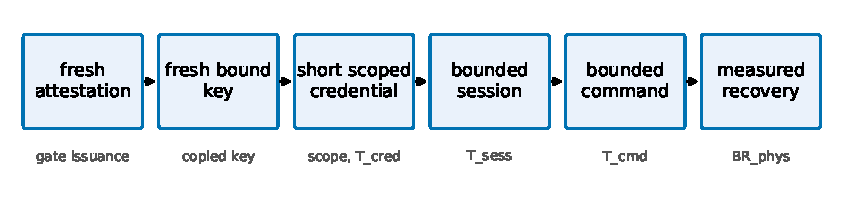
\includegraphics[width=\textwidth]{figures/fig_chain.pdf}
\caption{The CONTAINDER containment chain. Each link bounds a dimension: attestation gates
issuance, fresh-key binding contains a copied key, scope and short lifetime bound $\BRflex$ and
$T_{\mathrm{cred}}$, session and command enforcement bound $T_{\mathrm{sess}}$ and
$T_{\mathrm{cmd}}$, and measured recovery bounds $\BRphys$.}
\label{fig:chain}
\end{figure*}

\subsection{Components and trust layering}
The device keeps a long-lived, hardware-rooted bootstrap identity~\cite{ieee8021ar2018} used only for
enrollment and attestation, never accepted directly for DER control. An \emph{attester} produces
fresh evidence bound to a freshly generated operational public key; a \emph{verifier} checks
evidence against endorsement and reference values and returns an explicit result; a
\emph{credential issuer} signs a short-lived operational certificate embedding role, site, scope,
and expiry only for a valid attestation result; an \emph{authorization service} maps the
operational identity to least-privilege function-set assignments; the \emph{2030.5 server or
proxy} authenticates the operational certificate, enforces a maximum session age, and rechecks
authorization per command or at a bounded interval; a \emph{session controller} and a
\emph{command-lifecycle controller} bound authority beyond expiry; and a \emph{risk controller}
selects deny, scope narrowing, or bounded emergency renewal. We use the Entity Attestation
Token~\cite{rfc9711} under the RATS Attester/Verifier/Relying-Party model~\cite{rfc9334}, and
define a concrete EAT profile rather than treating EAT as a complete attestation protocol.

\subsection{Fresh-key binding}
Attesting a device is not sufficient: a healthy device can pass attestation while an attacker
retains a previously copied operational key. CONTAINDER therefore requires that every credential
epoch use a newly generated operational key, generated in a TPM, TEE, or secure element where
available and marked non-exportable, whose public-key digest is carried in the attestation
evidence. The issuer signs only the attested public key, refuses renewal that presents only a
prior certificate, rejects replayed evidence and reused nonces, and rotates the key even when the
device stays healthy. This is what contains a copied key across the next epoch.

\subsection{Session and command-effect enforcement}
Certificate expiry does not end an open TLS session or an already-issued long-duration control.
CONTAINDER closes sessions at credential expiry (or bounds session age to the credential TTL) and
revalidates authorization per command, and it bounds adversary-issued controls through a maximum
command duration, cancellation on containment, and safe-default restoration, with explicit
handling of scheduled DERControls. The two quantities the prototype measures are
\begin{align}
\Delta_{\mathrm{expiry}} &= t_{\text{last adv.\ command}} - t_{\text{expiry}},\\
\Delta_{\mathrm{effect}}  &= t_{\text{effect ends}} - t_{\text{expiry}},
\end{align}
each targeted to zero or a small declared bound. These are exactly the $T_{\mathrm{sess}}$ and
$T_{\mathrm{cmd}}$ components of $\BRauth$.

\subsection{Safe-mode policy}
Failure behavior is explicit rather than fail-open. The risk controller chooses among the states
in Table~\ref{tab:safemode}; no failure mode grants indefinite authority, and the safety of each
degraded state is validated under feeder conditions rather than assumed.

\begin{table}[t]
\centering
\caption{Safe-mode authorization states.}
\label{tab:safemode}
\small
\begin{tabular}{@{}p{0.24\columnwidth}p{0.34\columnwidth}p{0.30\columnwidth}@{}}
\toprule
State & Allowed & Denied \\
\midrule
Healthy & normal scoped control & out-of-scope control \\
Verification delayed & read telemetry, hold last safe schedule & new high-impact dispatch \\
Attestation uncertain & read-only, bounded emergency control & arbitrary set-points \\
Known compromise & read-only or total denial & all control \\
Issuer outage & prior low-risk scope, bounded grace & scope expansion, high impact \\
\bottomrule
\end{tabular}
\end{table}

\subsection{Migration compatibility}
We separate three compatibility levels --- \emph{protocol} (2030.5 messages stay conformant),
\emph{implementation} (unmodified client or server software can participate), and \emph{deployment}
(legacy and upgraded devices coexist) --- and claim none of them without a passing interoperability
test rather than asserting ``backward compatible.'' None has yet been tested;
Section~\ref{sec:prelim} reports interoperability as untested. Three tiers realize this: a
bootstrap-only legacy tier, a gateway-attested proxy tier where an edge gateway holds the
operational credential for downstream legacy devices, and a native device-attested tier.

\subsection{What non-renewal inherits from the constraints it cites}
% Reviewer M11: the mechanism inherits at least two of the three deficiencies it cites against OCSP.

Section~\ref{sec:threat} adopts the Sandia analysis's reasons why online revocation fails for DER:
no guaranteed connectivity, no trustworthy time on inverters, and no responsible reporting party.
Our mechanism inherits two of the three, and we state that rather than let a reader find it.

\emph{Secure time.} Expiry is a judgment about time, so an endpoint that cannot trust its clock
cannot enforce a short lifetime --- the deficiency cited against OCSP --- and a skewed device
clock would extend a ``short-lived'' credential indefinitely. So \textbf{expiry is never enforced
by the endpoint alone}: the issuer refuses renewal server-side where a trustworthy clock exists,
each renewal binds a fresh key to a verifier-supplied nonce so a replayed attestation cannot
extend authority however the clock reads, and session and command limits are monotonic counters
rather than wall-clock deadlines. A skewed clock then costs availability, not containment. We
have not measured skew.

\emph{Connectivity.} A twelve-hour lifetime means a DER losing backhaul for twelve hours loses
control authority, and rural outages of that length are routine. An aggregator that drops a fifth
of fleet controllability during a verifier outage has created a reliability hazard while closing a
security one. Safe-mode degradation to an autonomous volt-var profile exists for this reason;
whether the trade is acceptable is an operator's call. Our availability figures come from
in-process injection, not networked outages, and renewal storms are untested.

\emph{Who reports compromise.} Attestation detects only what it measures. Firmware integrity is
measurable; \textbf{a stolen operational key on a device with intact firmware passes
attestation}. Per-epoch fresh-key binding answers this, but containment latency is then not the
lifetime: with per-cycle detection probability $p$ and lifetime $T$, expected retention is $T/p$
--- twelve hours at $T{=}6$\,h, $p{=}0.5$, and equal to $T$ only at $p{=}1$. \textbf{We report
$T/p$ as the containment-latency figure of merit.} The alternative, a narrow access list on a
long-lived credential, contains a copied key only when someone notices and edits the list, which
has no bounded latency at all. Bounded beats unbounded; it does not beat instant.

\emph{Which tier is deployable.} Presenting three tiers evenhandedly would mislead: only one is
deployable within the next standards cycle. The native tier needs attestation and a trusted clock
on constrained inverter hardware; the legacy tier changes nothing. \textbf{The gateway-attested
proxy tier resolves all three inheritances at once} --- the gateway holds the credential and the
clock, attestation runs on capable hardware, downstream devices stay unmodified, and short
outages are buffered --- and it alone requires no change to already-certified endpoints. We regard
it as the deployment path.

\subsection{Implementation status}
% provenance: mis_01KXT2D8VVC1CDNT9WJ4CFGH9P (M3 spec).
The design is realized as an issuance and renewal service using real X.509 certificates and mutual
TLS, with a Python IEEE~2030.5-style client in place of the EPRI C client and structured event
logging for every credential, session, and command transition. Its security invariants and
workstation overhead are reported in Section~\ref{sec:prelim}; a native EPRI-client integration and
constrained-hardware measurements remain future work.

\section{Cyber-Side Analysis Engine}
% provenance: M2 report (mis_01KXT2BS2S584NBFQAN2P4D6SK); implemented and tested.
% provenance: dec_01KXT240A70R8N104BPN5G07CJ (RQ1: reach attributable to scope vs authentication).

We implement the cyber-side impact dimensions as an analysis engine, \texttt{pkimodel}, that computes
$\BRreach$, $\BRflex$, and $\BRauth$ for a compromise locus under a policy. The engine models
the identity and delegation graph over the six node types of the threat model, with typed
issuance, delegation, and authorization edges. Its central modeling choice follows the
formalism: a credential's reach (which DERs it can address) is represented independently of
its scope (which function sets it may invoke at each DER). This is what makes the separating
counterexample expressible in code, and we ship that counterexample as a regression test:
the two compromises resolve to an identical reachable set of eleven DERs, yet the engine
computes zero commandable kW for the attested credential against tens of MW for the legacy
one, and a persistence of hours against the analysis horizon.

The authorization policy is parameterized, not fixed: a hardcoded permissive access model would
overstate what a stolen certificate can command, so the engine exposes four ACL realism levels
spanning single-device, site, feeder-segment, and whole-fleet scope, varied in the evaluation. On a
synthetic 200-device fleet over four feeders the reachable-DER count grows from one (single-device
and site) to fifty (feeder) to two hundred (fleet), with commandable capacity in step; the
feeder-level figure is the fleet divided by the feeder count and moves with that parameter. This
operationalizes RQ1: most reach gained by a compromise is attributable to authorization scope
rather than to authentication alone. Retained authority is returned as a distribution over
duration, not a point estimate, and separates credential, session, and command-effect components.

The engine consumes synthetic scenarios from a deterministic, seedable generator, since real
utility authorization graphs are not public; the generator is released as part of the
artifact. The engine is cyber-side only. It produces the reachable-DER set and the
commandable-capacity envelope that the feeder simulation consumes to compute $\BRphys$.

\section{Feeder Co-Simulation Methodology}
% provenance: mis_01KXT2DXXY862RPX7YATTRBDWB (M4 spec); dec_01KXT27V1Y4ZR6ZRAST3H94WC7 (testbed decision).
% provenance: dec_01KXT4C6ZPYD1Z92DH6CN1KKM3 (BR_phys unit = ANSI C84.1 excursion + trip flag).

The physical consequence radius is measured by a feeder co-simulation that translates an
authorized-control reach from the analysis engine into a malicious dispatch program and runs
it on a public distribution feeder. We take the IEEE 8500-node feeder as the primary
benchmark and the PNNL 9500-node system as an advanced validation tier. Time-series inputs
come from public solar and load datasets. This part of the work is methodologically routine
relative to the false-data-injection literature on distribution systems, so we build it to be
unimpeachable rather than novel.

Two choices harden it against the standard objections to simulation studies. First, we cross-
check OpenDSS against an independent GridLAB-D solver on the base case and on at least one
attack case, following the precedent of the PNNL 9500 report, and we report any divergence
rather than suppressing it. Second, credential state gates dispatch inside the co-simulation
through a HELICS federation, so that a denied or narrowed credential actually prevents a
command in simulation rather than being applied after the fact. The attack families are
volt-var curve distortion, volt-watt curve distortion, export-limit distortion, and
curtailment spam. The metrics are the count of nodes violating the ANSI~C84.1 bands, maximum
voltage deviation, the area under the violation curve over time, regulator tap operations,
unnecessary curtailment, energy not served, and recovery time to steady limits, with the
per-unit voltage excursion as the primary continuous measure and a protection-trip flag as
the discrete outcome.

We do not tune feeder parameters to amplify impact; we report what the standard models
produce. The clean base case, the four attack families, the eight metrics, and the
cross-solver agreement are the acceptance criteria for this component. As with the credential
service, a first benchmark run on the IEEE~8500-node feeder appears in the preliminary evaluation;
the full sweep on both feeders, with the GridLAB-D cross-check and seasonal operating states,
follows the pre-registered protocol chosen in advance.

\section{Evaluation Methodology}\label{sec:protocol}
% provenance: experiments/PREREGISTRATION_CONFIRMATORY.md, committed at git f35c2e7 before any
% treatment arm ran; amendments A1 and A2 recorded there.

\paragraph{What the pre-registration guarantees, and what it does not.}
The hypotheses, endpoints, operating ladder, authorization families, attacker models,
interpretation rules and exclusion policy are recorded in
\texttt{PREREGISTRATION\_CONFIRMATORY.md}, \textbf{committed to version control before any
treatment arm was run}. The ordering is checkable: the commit introducing that document precedes
the commit introducing every result file the paper reports. This is a genuine ordering guarantee
within the repository and it is what the predecessor version of this work lacked, since there
every result predated the repository itself.

It is not an independent timestamp. The commit is authored by the party who could rewrite history,
so it establishes ordering to a reader who trusts the repository and not to one who does not.
Converting it into an independent guarantee requires a third-party deposit, which has not been
made. We claim repository-internal ordering and nothing more.

\paragraph{Two departures, both disclosed.}
Before any result of the shape sweep was seen, the top rung of each penetration ladder and two
points of the attacker grid were removed: at those rungs the strong-injection admissible points
exhaust the solver's retry budget and the sweep projected four and a half hours. The first run was
stopped and its partial output discarded rather than merged, and both removed rungs sit beyond
their feeder's compliance transition and support no primary claim.

The second departure was made \emph{after} seeing results and is a defect correction. The IEEE~123
fleet had been set to $91$, exactly that feeder's load-bus count, so every seed selected the same
buses and merely permuted them: all twenty IEEE~123 seeds were one circuit, returning a single
distinct value per rung with degenerate bootstrap intervals. The nominal $n{=}20$ was an $n{=}1$.
This is the same class of error as the predecessor's withdrawn ablations --- replication reported
where the harness produced none --- and it is corrected the same way. The IEEE~123 fleet was
halved so that placement varies with the seed, those arms were re-run, and the originals were
discarded. IEEE~8500, whose $600$ units are drawn from $1177$ load buses, was unaffected. No
hypothesis, endpoint, interpretation rule or seed count changed.

One interpretation rule could not be applied as written, and \S\ref{sec:results} gives the
substitution and the null control that justifies it.

\paragraph{Statistics.}
The experimental unit is the complete paired scenario run --- (feeder, rung, set, primitive,
attacker, seed) --- never a node, a timestep or a command. Every contrast is paired on seed: the
same seeded fleet placement carries the legitimate baseline and every treatment arm at that seed,
and each arm is an independent compile so no solver state leaks between arms. Estimates are the
median paired difference with a bias-corrected percentile bootstrap interval at $10{,}000$
resamples; count outcomes additionally carry an exact binomial sign test. Twenty paired seeds
support every primary contrast. Holm correction is applied within each hypothesis family and not
across them.

Non-convergence is a recorded outcome, never a dropped run: the retry cap is two with the
control-iteration budget tripling $500 \to 1500 \to 4500$, unsettled solves are retained and
flagged, and every reported aggregate carries its flagged count. The calibration sweep records
that IEEE~8500 at $300\%$ penetration does not converge under the corrected characteristic even
after the full ladder, which is why the ladder stops below it.

\paragraph{Operating states.}
The ladder is calibrated, not assumed. A hosting-capacity sweep under \emph{legitimate} operation
only --- no treatment, no attacker --- locates the penetration at which each feeder's legitimate
volt-var operation stops holding the ANSI upper band, using a tolerance relative to that feeder's
own zero-PV base case, because the IEEE~8500 base is itself marginally out of band with no PV
present. The resulting limits are $50\%$ penetration on IEEE~8500 at half load and, on IEEE~123,
\emph{right-censored}: that feeder holds the band at every penetration tested up to $1200\%$,
because its voltages stay inside the characteristic's deadband. That censoring is why the
confirmatory ladder is an explicit penetration ladder per feeder rather than fractions of a limit,
and why \S\ref{sec:results} reports fleet reactive absorption alongside penetration --- it is the
quantity that actually varies with exposure.

\section{Preliminary Evaluation}\label{sec:prelim}
% provenance: jrn_01KXTX3PH43VR78AM1GZHC27T1 (real in-session results: credsvc + OpenDSS).
% All numbers here are measured, at reduced scale; the full pre-registered sweep remains future work.

We report a preliminary evaluation that exercises the full pipeline end to end and produces
measured results. Its scope is deliberately limited and stated plainly: a workstation platform
(no constrained hardware), the real IEEE~8500-node feeder as a first benchmark run but not yet the
PNNL 9500 system, a single solver (OpenDSS, no GridLAB-D cross-check), load-state snapshots rather
than a full seasonal time series, one PV penetration level, a fixed rather than per-state-optimized
attacker, and a Python IEEE~2030.5-style client in place of the EPRI C client. These results
establish that the mechanism and the measurement work; the pre-registered full-scale sweep is not
replaced by them. Table~\ref{tab:implstatus} states the status of each component.

\begin{table}[t]
\centering
\caption{Implementation and evaluation status.}
\label{tab:implstatus}
\small
\begin{tabular}{@{}p{0.62\columnwidth}p{0.28\columnwidth}@{}}
\toprule
Component & Status \\
\midrule
Cyber-side analysis engine & implemented, measured \\
Credential service (issuance, fresh key, session/command enforcement) & implemented, measured \\
Feeder co-simulation (OpenDSS, two feeders) & implemented, measured \\
Availability fault injection & implemented, measured \\
Native EPRI-client 2030.5 traffic & planned \\
Constrained-hardware / TEE attestation & planned \\
GridLAB-D cross-solver check & planned \\
Interoperability tests & planned \\
Full pre-registered sweep & planned \\
\bottomrule
\end{tabular}
\end{table}

\paragraph{Functional invariants and containment (C1, C2).}
The credential service uses real X.509 / ECDSA certificates and an EAT-style attestation token.
Ten implemented security invariants all pass: bootstrap identity cannot authorize control,
issuance requires a valid fresh attestation, the certificate is bound to a freshly generated
operational key, replayed evidence is rejected, an expired credential cannot issue commands,
per-command scope matches issuance, a bad measurement yields only a narrowed safe-mode scope, a
prior epoch cannot self-renew, and a copied prior operational key is contained at the next epoch.
With per-command revalidation the post-expiry acceptance gap is
$\Delta_{\mathrm{expiry}} = -0.5$\,s (the last accepted adversarial command precedes expiry),
against $+5.0$\,s without enforcement, where it grows to the cached session age. A fresh
operational key is generated each epoch, so a copied key is useless after rotation.
Table~\ref{tab:invariants} lists the invariants and their outcomes.

\begin{table}[t]
\centering
\caption{Security invariants (all pass on the prototype, real X.509/mTLS).}
\label{tab:invariants}
\small
\begin{tabular}{@{}p{0.06\columnwidth}p{0.74\columnwidth}c@{}}
\toprule
ID & Invariant & Result \\
\midrule
I1 & Bootstrap identity cannot authorize control & pass \\
I2 & Issuance requires a fresh attestation & pass \\
I3 & Credential bound to a fresh public key & pass \\
I4 & Replayed evidence rejected & pass \\
I5 & Expired credential cannot issue a command & pass \\
I6 & Scope enforced per command & pass \\
I7 & Bad measurement yields degraded/denied scope & pass \\
I8 & Prior epoch cannot self-renew & pass \\
I9 & Copied prior key fails after rotation & pass \\
I10 & Active session/command bounded past expiry & pass \\
\bottomrule
\end{tabular}
\end{table}

\paragraph{Overhead (C3).}
On the workstation tier, over 500 iterations (100 for the handshake), the median software-path
latencies (no hardware root of trust, no network transport) are
$0.015$\,ms for key generation, $0.05$\,ms for attestation construction, $0.2$\,ms for a full
attested issuance, and $1.1$\,ms for a real mutual-TLS handshake, with p99 tails within a few
milliseconds; the issuer sustains about $4900$ issuances per second single-threaded. Renewal is
therefore inexpensive on this platform. The measured operations are standard EC~P-256 primitives
dominated by a single ECDSA signature and verification, so per-issuance cost on a constrained
inverter controller can be estimated from its public-key throughput; a hardware-backed measurement
is declared future work rather than claimed here.

\paragraph{Availability (C6).}
Renewal is a full attested issuance, so its cost is the issuance cost above; the renewal safety
margin $T_{\mathrm{TTL}} - (T_{\mathrm{renew,p99}} + T_{\mathrm{net}})$ stays positive at every
tested lifetime down to five minutes, and a $100{,}000$-device fleet re-mints in about $20$\,s
single-threaded, so short lifetimes are latency-feasible. The availability risk is instead a
verifier or issuer outage longer than the credential lifetime. Injecting verifier outages into the
running service (renewal fails during the outage), fail-closed denial retains $0.77$ of legitimate
control availability over the outage window, a bounded grace period $0.83$, and degraded-scope safe
mode $1.0$; control recovers as soon as the verifier returns. The injection is in-process; a
networked or hardware outage, clock skew, and renewal storms remain for the full study.

\paragraph{Feeder consequence (C5).}
We run an export/overvoltage attack on the real IEEE~8500-node feeder (4876 buses, 1177 loads,
12\,MW) with 600 seeded rooftop-PV units, ten paired seeds, under three load states.
Table~\ref{tab:prelim} reports the attack-induced overvoltage-violation area $\Delta J_V$, the
median over seeds against the base case at the same load. Because the 8500 base has native
undervoltage at its extremities, we report the induced \emph{overvoltage} area the attack targets
rather than a two-sided area that would credit the attack for lifting sagging nodes; this
attack-specific endpoint was chosen after observing the base undervoltage, while the two-sided area
remains the declared primary system-level endpoint. Under light
load and high PV a legacy full-authorization compromise induces a median $\Delta J_V = 126.6$
(range $108$--$134$); the CONTAINDER narrowed scope keeps it within the ANSI band (median $\Delta J_V \le 0$). Under
normal load the figures are $6.6$ against $0.1$. Under heavy load the export attack cannot raise
voltage above the band, so $\Delta J_V \approx 0$ regardless of policy. The ephemeral-only baseline
equals the legacy one physically, since a short lifetime does not narrow scope; its advantage is
temporal. The consequence is strongly state dependent, the physical-state separation of
Proposition~3 on the real benchmark.

\paragraph{Time-series containment and mechanism decomposition (C5).}
% provenance: jrn_01KY13EQJ6V8AZCRHB944ZAZJY (real 8500 time-series).
To measure temporal containment directly, rather than as a product of a measured and a modeled
factor, we run each policy as one time-series: a compromised credential drives the DER from minute
five, and its lifecycle then determines whether the malicious setpoint keeps affecting the feeder.
We integrate the real induced overvoltage area over time, in p.u.-node-minutes
(Fig.~\ref{fig:timeseries}). A legacy credential (B1) holds the feeder in violation for the whole
horizon (integral $6956$, no recovery). Holding the broad scope fixed but adding the CONTAINDER
lifecycle (A4) halves the integral to $3196$ and the feeder recovers at credential expiry, which
isolates the temporal effect of lifetime with session and command enforcement at equal scope.
Removing session enforcement (A2) or command cleanup (A3) from that configuration returns the
feeder to no recovery ($7030$), so each mechanism is necessary. Narrowing scope (B5) additionally
bounds the instantaneous envelope, and the integral falls to $3.8$. This single experiment gives
the equal-scope decomposition the design intends: scope bounds the envelope, lifetime with
enforcement bounds the duration, and neither alone suffices.

\begin{figure}[t]
\centering
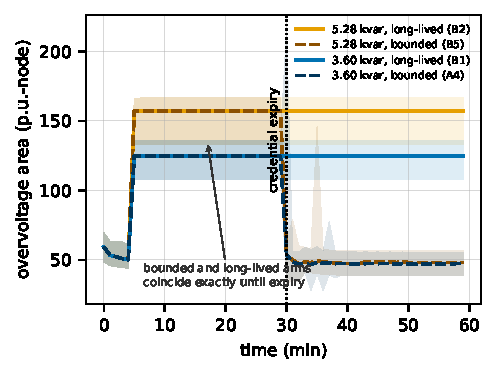
\includegraphics[width=\columnwidth]{figures/fig_timeseries.pdf}
\caption{Time-series induced overvoltage on the IEEE 8500-node feeder (light load, one seed).
A legacy credential (B1) never recovers; at the same broad scope the CONTAINDER lifecycle (A4)
recovers at credential expiry; narrow scope (B5) additionally bounds the instantaneous envelope.
The session-off and command-cleanup-off ablations track B1 and are omitted for clarity.}
\label{fig:timeseries}
\end{figure}

\paragraph{Policy comparison and the persistence--scope interaction (C5, H1).}
% provenance: jrn_01KXWJ4TPTK2DGSBKY5YCF50T5 (real 8500 full baseline + ablation sweep).
As a first-order summary that separates all six baselines at once, we also report a proxy
combining the measured physical envelope with the modeled retained authority,
$\Delta J_V \times \BRauth$ (Table~\ref{tab:exposure}); this is a physical-impact-times-duration
quantity, not the flexibility-time $\BRexp$ integral of the model, and the time-series above is the
direct measurement it approximates. At full authorization scope, lengthening persistence from the
ephemeral B3 (retained authority $\approx 10$\,h) to the legacy B1 ($\approx 2$\,years) multiplies
light-load exposure roughly $1700\times$, from $1.3\times10^3$ to $2.2\times10^6$. At narrow scope
the same change is inert: B2 and B5 are both near zero. The effect of persistence therefore
depends on scope, consistent with the pre-registered persistence-by-scope hypothesis; because
exposure is a product of a measured and a modeled factor, this preliminary pattern does not by
itself establish the pre-registered mixed-effects test over the full sweep. The full design B5 has lower exposure than both the ephemeral-only B3 and
the attestation-only B4 ($8.3\times10^3$), so neither half alone suffices. Mechanism ablations
attribute the reduction: removing scope narrowing restores physical exposure (from near zero to
$1.5\times10^3$), while fail-open renewal inflates retained authority from $12$\,h to
$1.75\times10^4$\,h. Scope narrowing bounds the physical envelope; attestation-gated renewal with
session and command enforcement bounds how long it persists, the temporal containment the C2
copied-key and session-theft results measure.

\begin{table}[t]
\centering
\caption{First-order exposure proxy $\Delta J_V\times\BRauth$ by baseline (light load, IEEE 8500, N{=}10; $\Delta J_V$ measured, $\BRauth$ modeled). The time-series (Fig.~\ref{fig:timeseries}) is the direct measurement.}
\label{tab:exposure}
\small
\begin{tabular}{@{}llcc@{}}
\toprule
Baseline & Scope & $\BRauth$ & Exposure \\
\midrule
B1 legacy full & full & $\sim$2\,yr & $2.2\times10^6$ \\
B2 ACL-narrow & narrow & $\sim$2\,yr & $\approx 0$ \\
B3 ephemeral-only & full & $\sim$10\,h & $1.3\times10^3$ \\
B4 attestation-only & reference & $\sim$14\,d & $8.3\times10^3$ \\
B5 full CONTAINDER & narrow & $\sim$12\,h & $\approx 0$ \\
B6 safe-mode & narrow & $\sim$12\,h & $\approx 0$ \\
\bottomrule
\end{tabular}
\end{table}

\begin{table}[t]
\centering
\caption{Attack-induced overvoltage-violation area $\Delta J_V$ on the IEEE 8500-node feeder (median over 10 seeds).}
\label{tab:prelim}
\small
\begin{tabular}{@{}lcc@{}}
\toprule
Operating state & Legacy full (B1) & CONTAINDER (B5) \\
\midrule
light load / high PV & 126.6 & $-0.01$ \\
normal & 6.6 & 0.13 \\
heavy load & $\approx 0$ & $\approx 0$ \\
\bottomrule
\end{tabular}
\end{table}

\begin{figure}[t]
\centering
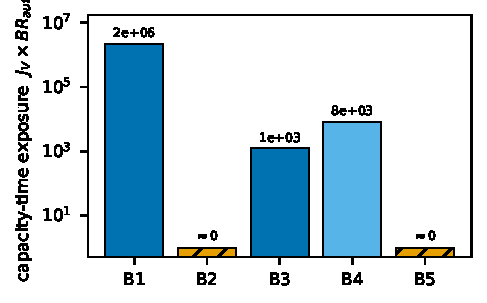
\includegraphics[width=\columnwidth]{figures/fig_exposure.pdf}
\caption{Capacity-time exposure by baseline on the IEEE 8500-node feeder (light load, log scale).
Persistence multiplies exposure only at full scope (B1 vs B3); at narrow scope (B2, B5) it is
inert, the persistence--scope interaction. Bars floored at 1 for log display; B2, B5, B6 are $\approx 0$.}
\label{fig:exposure}
\end{figure}

\begin{figure}[t]
\centering
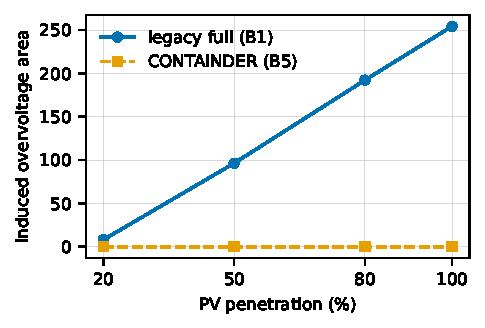
\includegraphics[width=\columnwidth]{figures/fig_penetration.pdf}
\caption{Induced overvoltage area versus PV penetration (IEEE 8500, light load, 5 seeds). Harm
scales with penetration under the legacy baseline; containment is penetration-independent under
CONTAINDER.}
\label{fig:penetration}
\end{figure}

\begin{figure}[t]
\centering
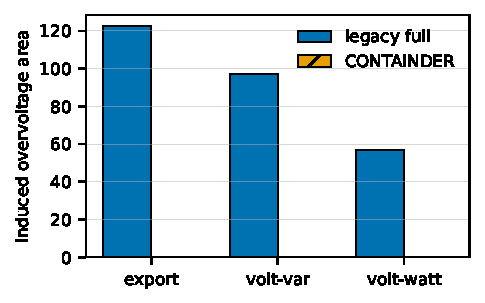
\includegraphics[width=\columnwidth]{figures/fig_attack_families.pdf}
\caption{Induced overvoltage area by attack family (IEEE 8500, light load). Narrowing scope
contains overvoltage driven by active or reactive authority.}
\label{fig:families}
\end{figure}

\paragraph{Penetration and robustness.}
Induced overvoltage grows with PV penetration under a legacy full-authorization compromise, from
$8$ at $20\%$ to $254$ at $100\%$, while the CONTAINDER narrowed scope holds it near zero at every
level (Fig.~\ref{fig:penetration}). The same containment holds across attack families
(Fig.~\ref{fig:families}), and capacity-time exposure separates all six baselines along the
persistence--scope interaction (Fig.~\ref{fig:exposure}). It also holds on a second public feeder:
on the IEEE~123-bus system a legacy full-authorization compromise induces overvoltage under high PV
penetration (induced area up to $2.2$) that CONTAINDER holds at zero, though the stiffer regulated
$4.16$\,kV feeder requires higher penetration than the 8500 to breach the band, consistent with the
feeder-dependence of Proposition~3.

\paragraph{Attack families.}
% provenance: jrn_01KXWJDXAC3N56E0477DDH5MMD (real 8500 attack-family sweep).
The containment holds across attack families, not only the export attack (five seeds, light
load). A legacy full-authorization compromise induces overvoltage areas of $122$ (export-limit),
$97$ (volt-var, reactive injection alone), and $57$ (volt-watt, active injection) that the
CONTAINDER narrowed scope reduces to zero in every case; for a curtailment-spam attack, narrowing
cuts the per-node voltage variability from $0.012$ to $0.004$\,p.u., a factor of three.
Overvoltage is reachable through active or reactive authority, and narrowing scope removes both.

\paragraph{Least privilege preserves legitimate utility (C5).}
A scope that removed all control would contain the attack trivially, by disabling the device.
CONTAINDER's operational scope is bounded volt-var support, not read-only. Under it a legitimate
reactive voltage-support command is authorized while an active-power export command is denied; the
attacker's only remaining lever is bounded reactive, which induces overvoltage $0.04$ against $126$
under full authorization, whereas a read-only scope authorizes neither the legitimate nor the
malicious command. The narrow scope therefore retains the most common legitimate DER function while
bounding the attack, which distinguishes least privilege from denial of service.

\paragraph{Limitations.}
These results are preliminary and we do not generalize them. Physical results come from two public feeders
(a ten-seed IEEE 8500 sweep and a confirmatory IEEE 123 run) and a single solver, with a fixed
export attacker; the IEEE 9500-node system was obtained
but did not converge in our OpenDSS build and is deferred to an appendix tier per the study's
pre-registered contingency. Retained-authority figures are model outputs under assumed attestation
and lifetime parameters, not measured field values, and the exposure metric inherits those
assumptions. The availability results model the outage response rather than injecting real verifier
outages on hardware. Incremental deployment is by construction; interoperability against an
unmodified endpoint is untested. The pre-registered sweep on two public feeders, with a
cross-solver check, seasonal states, constrained hardware, and the full seed budget, is what would
support quantitative claims; the 8500-node results are the primary feeder evidence here.

\section{Related Work}
% provenance: jrn_01KXT4CF02R1VRTMK9M3XQ6SEC (Passos differentiation); dec_01KXT28WTZ92PJ7S8D3MME78D4 (novelty framing).
% All citations verified against Crossref/OpenAlex/DBLP/IETF/publisher; no placeholders remain.

Table~\ref{tab:relatedcmp} compares CONTAINDER against the concrete systems and standards that
answer parts of the same problem, rather than against categories of work.

\emph{Workload identity is the closest existing system.} SPIFFE and its SPIRE
runtime~\cite{spiffe-spec,spiffe-cncf} implement almost exactly the chain we describe: attest node
and workload, issue short-lived scope-bound X.509 SVIDs keyed to the attested identity, refuse
renewal when attestation fails, rely on expiry rather than revocation. Recent work extends it to
IoT fleets~\cite{bakoyiannis2025spiffe} and nested tokens~\cite{cochak2024lsvid}. The question is
therefore whether CONTAINDER is workload identity with a DER label, and two differences are
load-bearing. First, SPIFFE has no notion of a \emph{physical effect that outlives the
credential}: withdrawing a workload identity stops a process opening new connections, but it does
not retract a volt-var curve already written into an inverter. Our $T_{\mathrm{sess}}$ and
$T_{\mathrm{cmd}}$ enforcement exists because actuation persists in a way computation does not,
and Section~\ref{sec:results} measures how far each layer reaches. Second, scope binds to
\texttt{FunctionSetAssignments}, whose conformant settings are dictated by
IEEE~1547-2018~\cite{ieee1547-2018} and CSIP~\cite{sunspec2018csip} rather than chosen freely.

\emph{The Web PKI has already adopted non-renewal.} The CA/Browser Forum defined a Short-lived
Subscriber Certificate in 2023 and \emph{exempted it from CRL and OCSP status
checking}~\cite{cabf-sc063v4} --- ``non-renewal replaces revocation'', already ratified, with
Baseline Requirements v2.2.8 setting the threshold at seven days~\cite{cabf-br} --- and ballot
SC-081v3 phases maximum TLS validity from 398 days to 47 by 2029~\cite{cabf-sc081v3}. This is at
once the strongest external validation of the premise and the sharpest limit on our novelty. We
claim none for short-lived credentials or for expiry-based containment. The same limit applies
inside our own problem domain: the Sandia analysis of the DER standards recommends limited-life
certificates and states that manufacturers following the IEEE~2030.5 guidance are ``not required
to limit the life of a device certificate''~\cite{obert2019recommendations}, which makes a
short-lived operational credential \emph{permitted} rather than novel. What we claim is the
mapping onto DER authorization: which scope object to bind, which control point to withhold, and
that session and command-effect enforcement are separately necessary because grid actuation
persists.

\emph{Competing key management for power systems.} IEC~62351 is the sharpest comparison: Part~8
gives role-based access control~\cite{iec62351-8} and Part~9 specifies key management
\emph{including} enrollment and revocation for power-system equipment~\cite{iec62351-9}. Part~9 is
a directly competing answer, and the honest question is why 2030.5/CSIP does not adopt it. Not
technical superiority on our side: 62351-9's revocation machinery assumes the connectivity and the
responsible reporting party that the Sandia analysis found
absent~\cite{obert2019recommendations}, and CSIP deployments certify against the 2030.5 profile.
Where an operator has that connectivity, 62351-9 is a reasonable alternative, and we say so rather
than claim the field. IEEE~1547.3-2023 is the cybersecurity guide for interconnected
DER~\cite{ieee1547.3-2023} and the natural home for these recommendations;
NISTIR~7628~\cite{nistir7628r1} and IEC~62443~\cite{iec62443-3-3,iec62443-4-2} give the enclosing
frameworks; NREL's DER certification line~\cite{nrel80581,saleem2022dercert} and gap
analysis~\cite{magill2026dergap} document the certification landscape.

\emph{IEEE~2030.5 and CSIP security.} The 2018 and 2023 editions mandate mutual TLS with X.509
device certificates~\cite{ieee20305-2018,ieee20305-2023}, constrained for interconnection by
CSIP~\cite{sunspec2018csip}. The closest prior work is the 2030.5 security tutorial of Passos et
al.~\cite{passos2025tutorial}, a survey that proposes no redesign, quantifies no feeder
consequence, and formalizes no impact metric; Qi et al.\ survey the broader DER and smart-inverter
surface~\cite{qi2016cybersecurity}.

\emph{DER and smart-inverter attacks.} High-wattage IoT botnets can move the
grid~\cite{soltan2018blackiot,shekari2022madiot}; inverter attacks destabilize grid and
market~\cite{hui2025destabilizing}; distribution voltage control is attackable under high
PV~\cite{isozaki2016detection}; and the SUN:DOWN disclosure catalogs fleet-scale inverter
vulnerabilities~\cite{forescout2025sundown}. We tie the attack surface to the credential lifecycle
rather than assuming device compromise. Distribution-grid consequence is quantified by the
false-data-injection literature~\cite{liu2009false,deng2017false,liang2017review}, grounded by the
2015 Ukraine incident~\cite{liang2017ukraine} and quantitative risk
formulations~\cite{teixeira2015secure}; our feeder method is supporting, not novel.

\emph{Building blocks.} ACME~\cite{rfc8555} and Let's Encrypt~\cite{aas2019letsencrypt} automate
issuance, SCEP~\cite{rfc8894} is the incumbent device enrollment, and HTTPS-ecosystem measurement
quantifies the lifecycle problem~\cite{durumeric2013analysis}. Secure device
identity~\cite{ieee8021ar2018}, firmware TPM~\cite{raj2016ftpm} and hardware
DICE~\cite{jager2020dice} root the bootstrap layer; the RATS architecture~\cite{rfc9334}, the
Entity Attestation Token~\cite{rfc9711} and BRSKI~\cite{rfc8995} carry attestation, on established
principles~\cite{coker2011principles}. Web-PKI revocation delivery is
gap-ridden~\cite{liu2015endtoend}, scalable revocation remains
open~\cite{larisch2017crlite,smith2020letsrevoke}, and OCSP Must-Staple adoption is
weak~\cite{chung2018ocsp}. Attack-graph metrics~\cite{ou2005mulval,ammann2002scalable,
jajodia2005topological,wang2008attackgraph,frigault2008measuring,poolsappasit2012dynamic,
wang2014kzero} inform the notation of Section~\ref{sec:formalism}, which we do not claim as a
contribution. On the power side, IEEE~1547~\cite{ieee1547-2018} defines the DER functions, DERMS
perform feeder voltage management~\cite{rahman2021derms}, role-based access
control~\cite{sandhu1996rbac} abstracts the scoping we narrow, and HELICS~\cite{hardy2024helics,
palmintier2017helics} and GridLAB-D~\cite{chassin2008gridlabd} are the co-simulation tooling a
cross-solver check would use.

\begin{table*}[t]
\centering
\caption{Positioning against the concrete systems and standards that answer part of the same
problem. \emph{Short-lived} = credential lifetime is the containment mechanism; \emph{Attested} =
issuance is gated on fresh evidence about the endpoint; \emph{Numeric scope} = the authorization
can bound the \emph{value} a control may take, not only which function may be invoked;
\emph{Session expiry} = an established session stops accepting commands when the credential
authorizing it expires; \emph{Command cleanup} = an already-issued control is retracted;
\emph{Physical eval.} = consequence is evaluated on a power-flow model.
y = yes, n = no, p = partial, --~= not applicable.}
\label{tab:relatedcmp}
\footnotesize
\begin{tabular}{@{}p{0.27\textwidth}ccccccc@{}}
\toprule
System or standard & DER/2030.5 & Short-lived & Attested & Numeric scope & Session expiry &
Command cleanup & Physical eval. \\
\midrule
IEEE 2030.5 / CSIP baseline~\cite{ieee20305-2018,sunspec2018csip} & y & n$^{\dagger}$ & n & n & n & n & n \\
SPIFFE / SPIRE~\cite{spiffe-spec,spiffe-cncf} & n & y & y & n & p$^{\ddagger}$ & -- & n \\
BRSKI~\cite{rfc8995} & n & p & y & n & n & -- & n \\
CA/B Forum short-lived certs~\cite{cabf-sc063v4,cabf-br} & n & y & n & n & n & -- & n \\
IEC 62351-8 (RBAC)~\cite{iec62351-8} & p & n & n & p & n & n & n \\
IEC 62351-9 (key mgmt)~\cite{iec62351-9} & p & p & n & n & n & n & n \\
\textbf{CONTAINDER (this work)} & y & y & p$^{\S}$ & y & y & y & y \\
\bottomrule
\end{tabular}
\\[2pt]
{\footnotesize
$^{\dagger}$Device certificates have indefinite lifetime and CRL/OCSP are prohibited for
IEEE~2030.5 certificates; local allow/deny listing is permitted but not
required~\cite{obert2019recommendations}.
$^{\ddagger}$SVID rotation bounds new connections; SPIFFE defines no retraction of an effect
already actuated, because a workload has none.
$^{\S}$Partial: the attestation path is implemented and tested but software-emulated. No
hardware-backed key or attestation-quote measurement is reported (Section~\ref{sec:limits}).}
\end{table*}

\section{Ethics and Responsible Disclosure}
% provenance: mis_01KXT2D8VVC1CDNT9WJ4CFGH9P scope boundary (synthetic keys only; no production testing; no vendor-bound exploit tooling).

This work studies the consequences of credential compromise in order to bound them, and it
carries a corresponding responsibility. All experiments use synthetic and lab-generated
certificates. We use no real vendor keys or secrets, we test against no production DER fleet
or any internet-reachable device, and we build no exploit tooling bound to a specific vendor
product. The malicious dispatch programs exist only inside the feeder co-simulation and are
never emitted to hardware.

The physical-consequence results describe what a compromised but protocol-conformant
credential can already do under the deployed standard; they do not introduce a new
vulnerability so much as measure an existing exposure that the standard's prohibition on
revocation leaves unmitigated. Where results identify a concrete deployment weakness, we will
follow coordinated disclosure with the relevant standards body and affected implementers
before public release, and we will time any artifact release accordingly. The redesign and
its migration path are offered as the constructive counterpart to the measurement: the point
of quantifying the blast radius is to shrink it.

\section{Limitations and Conclusion}
% provenance: OUTLINE.md status column; jrn_01KXT4NN8Z8EG0SZYGB65H2T5J (venue); chk T1.1 open item.

\paragraph{Limitations.}
The boundaries of the evaluation are stated next to the results they bound, at the end of
Section~\ref{sec:prelim}: one feeder and a single solver, one PV penetration level at the
conformant scope envelope, modeled rather than measured retained authority, workstation-only
overhead, in-process availability injection, untested interoperability, an unmeasured
stealth-constrained attacker, and no access to the 2023 edition of the standard. Two further
boundaries belong to the model. The authorization graphs used by the engine are synthetic, because
real utility authorization graphs are not public; we mitigate this with a released parameterized
generator and by ablating access-model permissiveness rather than fixing it. And our claims about
revocation rest on the Sandia analysis rather than a clause-level reading of the edition in force.

\paragraph{Conclusion.}
Credential compromise in IEEE~2030.5 is not well described by how many nodes an adversary reaches.
It is described by how much physical capacity those nodes command, how long the adversary keeps
it, and what the feeder does in response. Our central empirical finding is about the \emph{shape} of the
authorization an operator grants, not about how tightly it is drawn. \textbf{On the
IEEE~8500-node feeder, a reactive authorization that permits zero absorption does not contain a
credential compromise, and one that mandates a floor on absorption does.} An adversary needing no
injection authority at all --- commanding zero, which sits inside any magnitude bound --- drives
the feeder past an overvoltage trip threshold in every seed, because withdrawing the volt-var
absorption is itself the attack. An adversary confined instead to a band holding at least about
three quarters of the conformant Category~B absorption trips no seed. Least privilege works here,
but only when the bound is a floor rather than a ceiling.

We expected the control primitive to be what separated these cases and it is not: we ran the sweep
under both a fixed-setpoint override and a bounded volt-var curve, and over the band an operator
would authorize the two are indistinguishable on the trip outcome. Reporting a primitive-level
separation would have described the shape of the two authorized sets we chose rather than anything
the feeder did, so we do not. Whether the standard's function sets can express an absorption floor
for a fixed setpoint is a question about IEEE~2030.5 that we could not answer without the edition
in force, and we leave it flagged as a conjecture in Section~\ref{sec:prelim}.

Two things follow. The concrete one is a recommendation to the standard's users: authorize a
reactive band that excludes zero absorption, by whichever function set carries it. The
second is that scope discipline remains insufficient on its own at the envelopes deployments
actually grant today, so bounding the \emph{duration} of retained authority still matters, and
that is what attested short-lived credentials with session and command-effect enforcement
provide. The price is stated rather than hidden: containment latency is the credential
lifetime divided by the per-cycle attestation detection probability, not the lifetime itself, and a
gateway-proxy tier is the only one of our three deployment tiers that resolves the secure-time and
constrained-hardware constraints the mechanism inherits from the problem it addresses. These are
pilot results on one feeder; the pre-registered confirmatory sweep is what would generalise them.


\section*{Data availability}
The analysis engine, the X.509/mutual-TLS credential service, the OpenDSS feeder experiment
scripts, the pre-registered scenario matrix with its recorded hash, and the result files supporting
this study will be released in a public repository upon publication. The IEEE~8500-node and
IEEE~123-bus test feeders used in the evaluation are publicly available from the referenced OpenDSS
distributions.

\section*{Declaration of competing interest}
The author declares that he has no known competing financial interests or personal relationships
that could have appeared to influence the work reported in this paper.

\section*{CRediT authorship contribution statement}
\textbf{Huan Bui:} Conceptualization, Methodology, Software, Validation, Formal analysis,
Investigation, Data curation, Writing -- original draft, Writing -- review and editing,
Visualization.

\bibliographystyle{elsarticle-num}
\bibliography{refs}

\end{document}
